\begin{minipage}[t]{170mm}
\vspace{3mm}
\begin{center}
\section*{Befriet af dværge!}
\emph{Hej-Ho}

Her er Ereborg, DBC sender til MatCamp 

\emph{Hej-Ho}

I hører os i stridsøksebåndet. 

Vi begynder med krignyhederne for Campen, herefter Dværgerådets proklamationer, de udencampske nyheder i øvrigt, en skildring af forholdende på Campen og en beretning om feernes sammenbrud på GDC.

Der foreligger endnu ikke nogen officiel meddelelse fra dværgenes side, om hvor lamngt Gimlis styrker er nået op i Vandrehallen. Campens presseansvarlige i fysiktårnet havde kl. 7 direkte kontakt med matlab og på dette tidspunkt havde Gimlis tropper endnu passeret døren til trappeopgangen. Det meddeles at de små styrker tidligt i nat startede deres fremrykning fra fysikbadene på vej mod campens undervisningslokaler. En øksekolonne nåede i nat døren med kortlæseren ved grænsen mellem fysik og matematik og fire meter fra vandrehallen. I de senest indløbende dværgefrontberetninger hedder det at situationen er så forvirret, at der ikke er nogen officiel nyhed om, hvor langt dværgene er nået. Campens presseansvarlige meddeler videre i sit telegram kl. 7: Store deltagermængder samler sig i vandrehallen, alle laboratorietimer er aflyst, alle sociale møder udsat og hele deltagerskaren venter utålmodigt på at give Gimlis øksebærere en hjertelig velkomst.

Der er på Campen en tioltagende følelse af, at der forhandles mellem dværgenes arme og tandfeen og den gode fe, og at der vil blive afsluttet en aftale om overgivelse. Denne formodning støttes af den kendsgerning at feerne har erklæret kemi og biologi for åbne institutter. Det synes ikke fornuftigt for feerne frivilligt at opgive den temmelig stærke forsvarslinje ved kemi og så derefter at kæmpe på matematik.

Der er stor nervøsitet blandt feernes tropper. Nogle steder ser det ud som om de er ved at forberede sig til kamp. For eksempel har de bemandet befæstningerne ved sodavandsautomaterne foran matlab, men adskillige andre steder er feerne øjensynligt utålmodige efter at komme til at overgibe sig. 

Fysisk sekretariat har videregivet forlydender om at hobitternes kaffebryggere skulle være landet på matematisk bibliotek og i dag gik der rygter på campen om at hobitter har sneget sig ned ad trappen. Alle disse rygter savner enhver begrundelse.

I nat blev der kæmpet voldsomt i matlabs hyggehjørne, rundt om spilbordet og der hørtes endog fingerknips. På matematisk bibliotek og på læsepladserne på anden sal havde fetropper været i indbyrdes regulær kamp.

\emph{længere pause}

I dette øjeblik meddeles det, at Gimli har oplyst, at feernes tropper i D- og E-bygningen og på Matcamp har overgivet sig. Her er Ereborg. Vi gentager: Gimli har i dette øjeblik meddelt, at feernes tropper i D- og E-bygningen og på Matcamp har overgivet sig.

\emph{pause}

Vi fortsætter nu udsendelsen med at oplæse de to proklamationer, som Campens frihedsråd udsendte i nat, altså inden den meddelelse vi netop har giver:

'Hvad enten der kommer til kamp eller kapitulation, vil befrielseskampens sidste timer kræve endnu større disciplin og selvbeherskelse end hidtil. Ingen gruppe må gå til handling, før ordrenen er givet. Algebraikere, analytikere, vi stoler på jer.'

Feerne kom altså til fornuft og valgte kapitulationen. Det var en af de muligheder, campens frihedsråd havde forudset i den proklamation, som vi netop har hørt og som blev forfattet i nat. Nu for nogle få minutter siden erfarede vi fra Gimlis hovedkvarter, at fjenden i D- og E-bygningen og på campen har kapituleret.

\emph{Den kanoniske matematikersang og Jeg er en matematiker fra HCØ afspille}
\vspace{3mm}
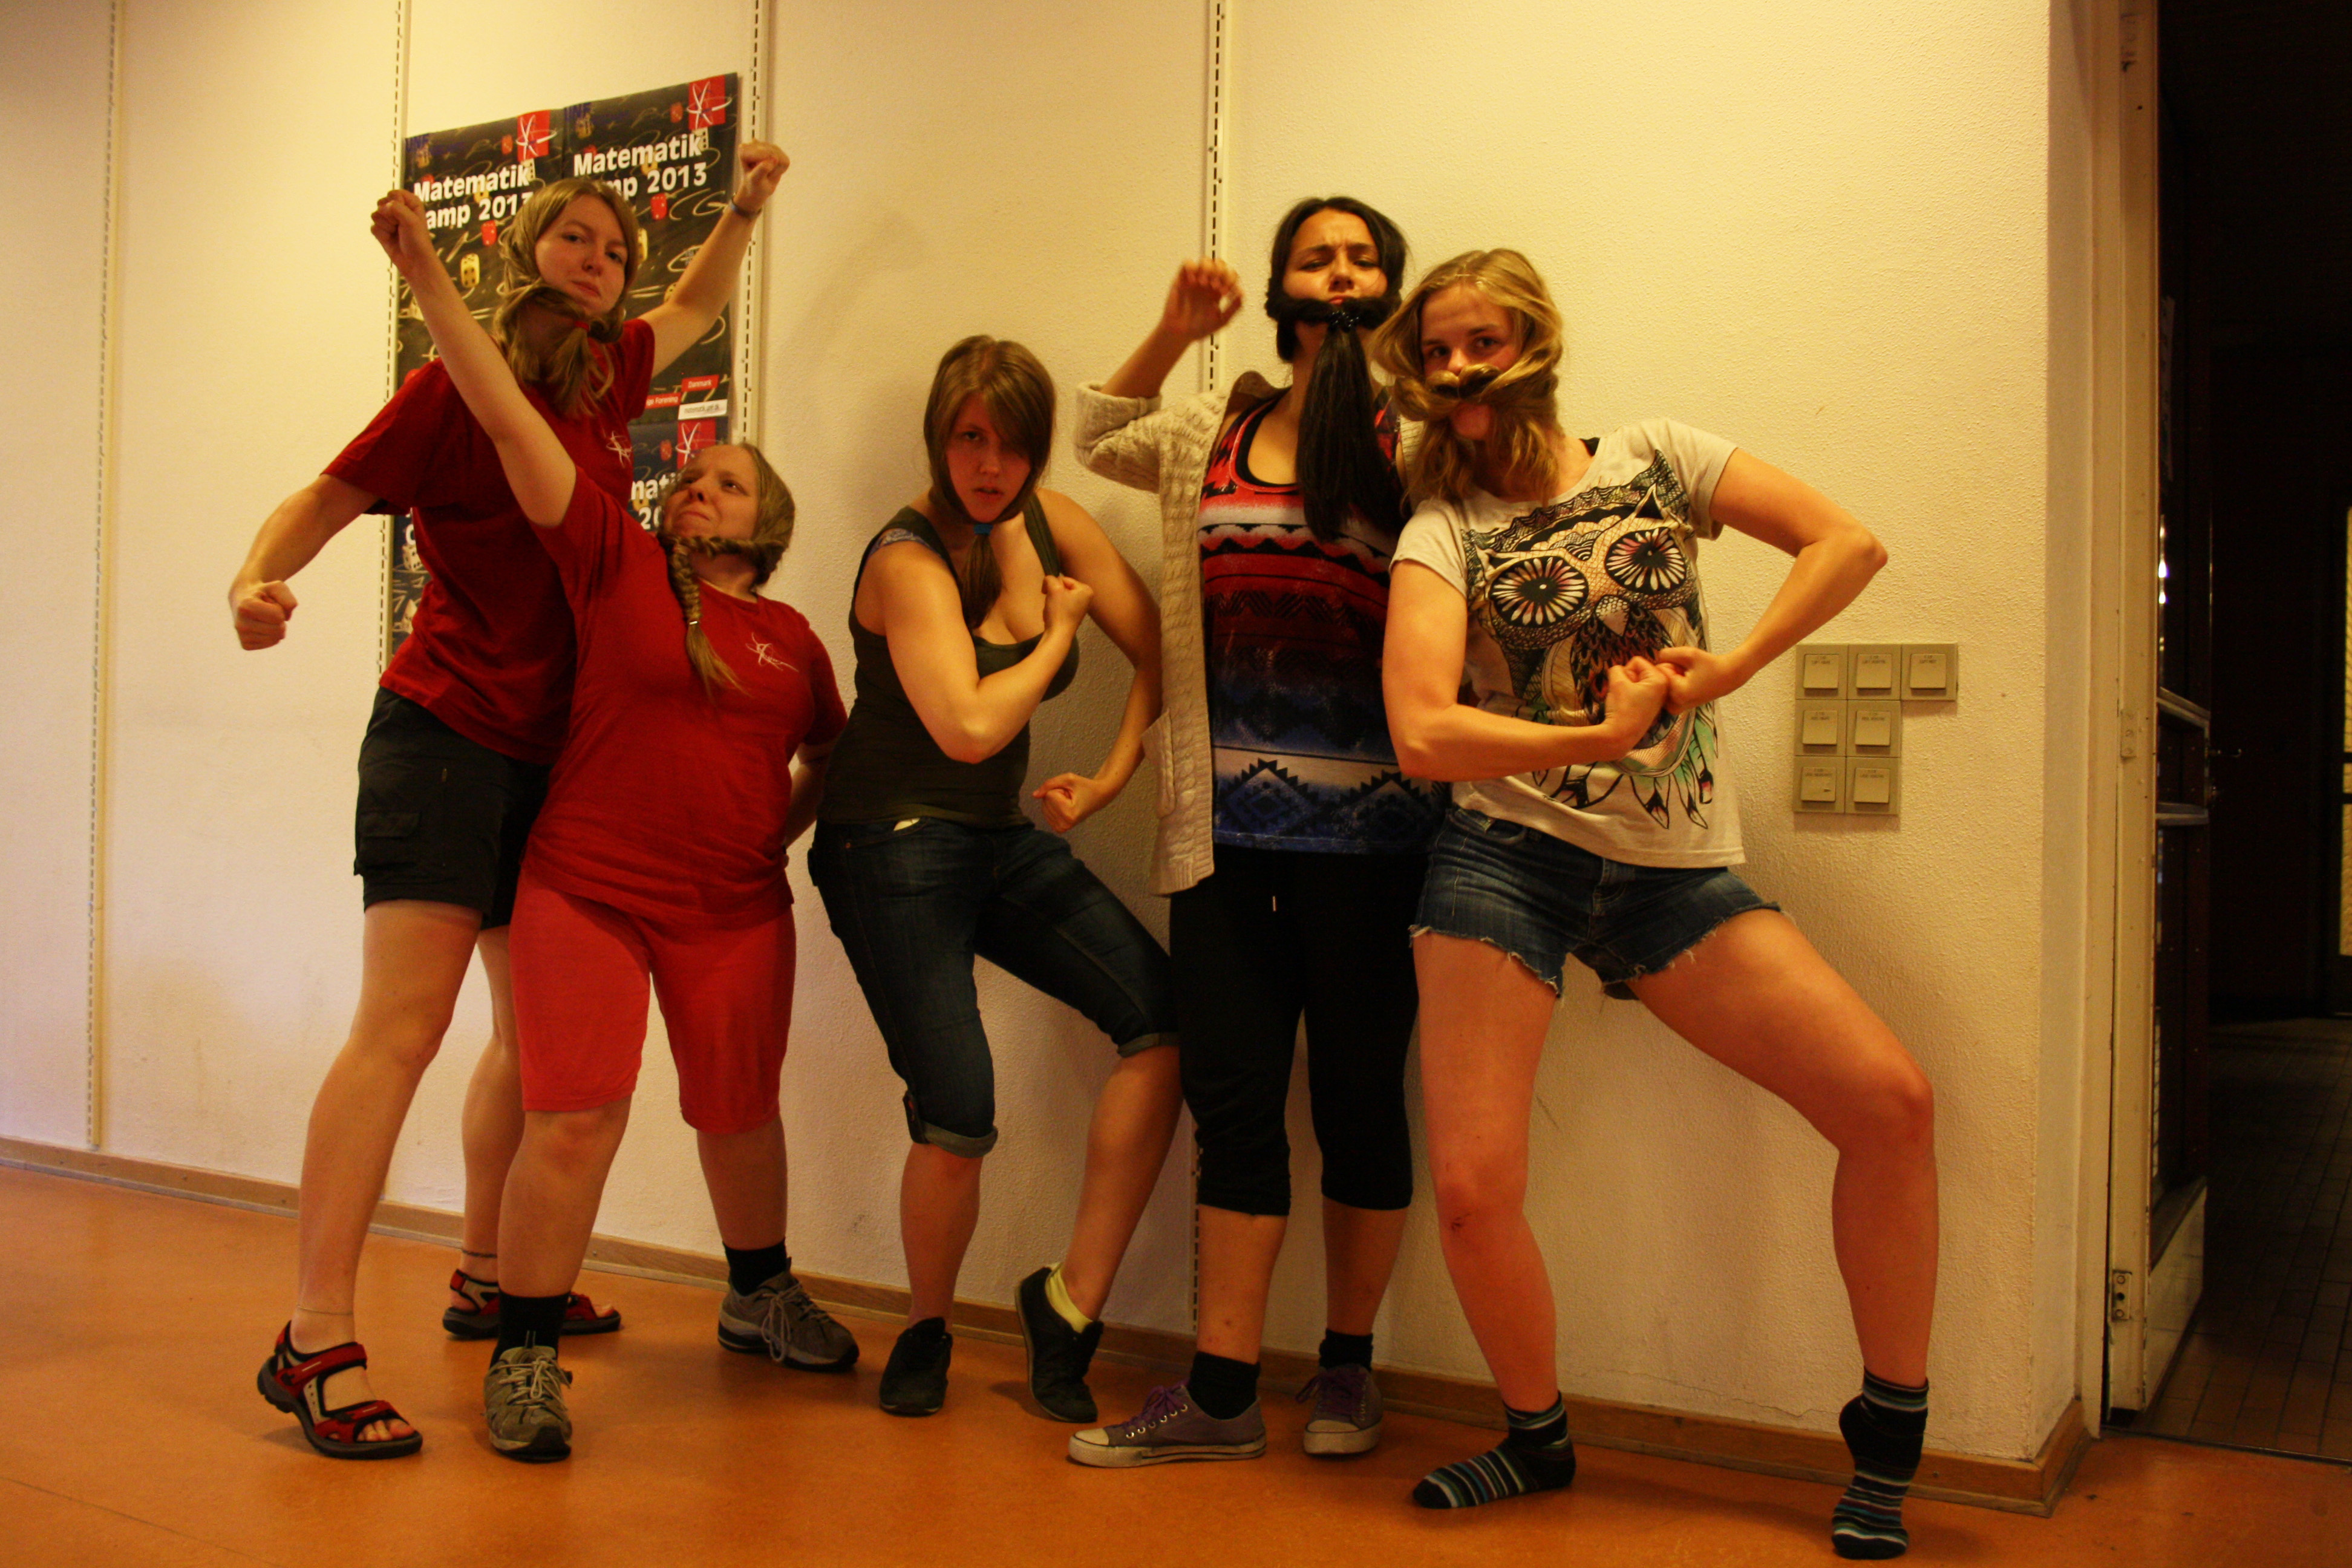
\includegraphics[width=130mm]{dvaergetropper.jpg}
\end{center}
\end{minipage}
